\chapter{Problem analysis}\label{cha:problemanalysis}
This chapter details the problem analysis, from the initial problem towards a problem statement. Based on the initial problem, a set of questions to research during the problem analysis has been determined:

\begin{description}
    \item[Arduino] What is Arduino, and who uses it? What is the Arduino programming language?
    \item[Concurrency] What is concurrency, and what does it mean to work concurrently? What are the different approaches/models for concurrency, and what are the challenges in relation to Arduino?
\end{description}

\section{Arduino}\label{sec:arduino}
Arduino is an open-source electronics platform that enables users to quickly create small microcontroller projects through easy-to-use hardware and software \cite{WhatArduino}. Multiple variants of Arduino boards exist, with different components and specifications. The UNO, Due, Mega2560, Micro, Leonardo, Zero, Mini, and UNO WiFi are within the classic family of Arduino boards. Because of Arduino being an open-source project, other companies are free to use the specifications to provide third-party implementations of the boards.

\todo{Kig på første sætning}
An Arduino UNO is used as the reference board for this project because \gls{aau} has provided one. All physical tests and examples will run on this board, and the implementation will depend on the Arduino UNO specification henceforth.

The software for the Arduino is the official Arduino IDE, in which developers can write code in the Arduino programming language. The IDE and the programming language is built on Wiring, which builds on Processing \cite{WhatArduino,WiringOrg}.

\subsection{The Arduino programming language}\label{subsec:arduinoprogramminglanguage}
The Arduino programming language closely resembles the C programming language and is, in fact, a set of C/C++ functions \cite{ArduinoSupportC}. It contains most of the constructs of C++, with some additional functions added and a few features, turned off in the compiler, such as exceptions \cite{Nongnuorg}.

\subsubsection{Sketches}
A program written in the Arduino IDE and programming language is called a sketch. A sketch follows a basic structure that consists of implementing the procedures "setup()" and "loop()". Setup is a procedure called once during a run - when the Arduino is turned on or reset; it initializes variables, pin modes, libraries, and some additional links. After setup, the loop begins. The loop procedure is a loop that runs for the duration of the runtime of the program and contains the logic of the project \cite{ArduinoLanguage}.

\subsection{Who uses the Arduino?}\label{subsec:whouses}
A wide range of people, such as students, hobbyists, children, programmers, and professionals, use Arduino for many different purposes \cite{WhatArduino}. Some are focused on the learning aspects of the Arduino - architecture, code, and embedded systems, while others are more interested in designing product concepts. Students and children can use the board to learn the basics of electronics; hobbyists may use it to build personal \gls{diy} projects, while professionals often use it to design product concepts \cite{WhatArduino}.

Designing a programming language for dedicated programmers or professionals may require a profound understanding of many underlying details of the Arduino platform itself. Providing a good language for these groups can potentially detract from the project's purpose - which is to design a programming language - because it may take more time than is available to obtain this knowledge. Thus, this is not the target group. The project also will not deal with a programming language designed for children, as this would require an understanding of pedagogical tools, which is outside the scope of a computer science education.

The hobbyist is, however, an excellent group for which to design our implementation for. Because hobbyists spend their leisure time on Arduino projects, the primary concerns are their limited available time and the potential for frustration during a project. Moreover, hobbyists might have limited programming proficiency or be complete beginners. The standard Arduino language already alleviates many problems, but not in regards to concurrency. The user group for the remainder of this report is hobbyists who want to do as much as they can with their limited time and limited coding proficiency - specifically related to concurrency.
\section{Concurrency}\label{sec:concurrency}
The term concurrency is a general term for ways a computer system performs multiple tasks simultaneously. It covers the \textit{simulation} of multiple tasks running at the same time through process switching, as well as work done in parallel. To disambiguate, based on the definition:

\blockcquote{Bryant2016}{We use the term concurrency to refer to the general concept of a system with multiple, simultaneous activities, and the term parallelism to refer to the use of concurrency to make a system run faster.}

We infer that parallelism is a type of concurrency to speed up the system, while concurrency, in general, may have purposes not related to speed, for example, synchronization of tasks.

Concurrency is a complex, large, and hardware-dependent subject~\cite{Sebesta2016}. The limitations of the Arduino hardware concerning concurrency, specifically the \gls{cpu}, are explored before concurrency in general because the project is, first and foremost, about programming language design - not concurrency.

\subsection{Arduino hardware}\label{subsec:arduinohardware}
The Arduino Uno board uses the ATmega328P microcontroller~\cite{ArduinoUno}. The architecture of this microcontroller is a scalar single-core processor without hyperthreading(intel) or \gls{smt} (AMD) equivalents~\cite{ATmega328P}.

Since there only exists a single core, which does not contain any duplicate copies of CPU hardware (for multithreading), the only hardware parallelism on the Arduino Uno is instruction-level parallelism, and only to the level of up to 1 instruction per clock cycle (scalar). This parallelism is also handled directly by the \gls{cpu} and does not impact the instruction set available to developers.


\begin{figure}[htb!]
    \centering
    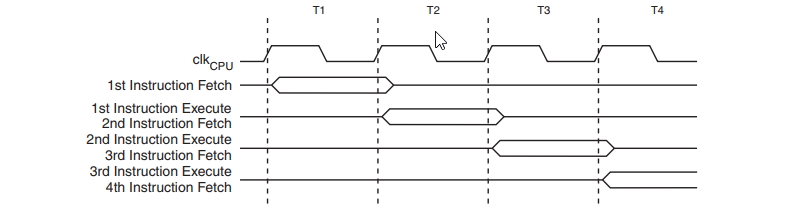
\includegraphics[width=\textwidth]{figures/Arduino_Pipeline.png}
    \caption{The parallel intruction fetches and intruction executions \cite{ATmega328P}}
    \label{fig:arduinopipeline}
\end{figure}


Therefore, the Arduino is a uniprocessor~\cite{Bryant2016} whose architecture does not support parallel processing - and for the remainder of the report, the term concurrency refers to concurrency \textbf{without parallelism}.

Even unicore processors can support several models for concurrency at the application software level, which makes sense since most computers often have more processes running than \glspl{cpu}. Achieving this concurrency is done through interleaving instructions of different processes, which lets the \gls{cpu} appear to run multiple programs.

This interleaving is commonly handled by an \gls{os}, which manages the hardware resources~\cite{Bryant2016}. However, by default, the Arduino does not have an \gls{os}. It is still possible to achieve concurrency on an Arduino, but not without a scheduler or scheduling.

\subsection{Concurrency on an Arduino}\label{subsec:concurrencyinarduino}
The scheduler is the part of the \gls{os} that handles the planning and switching of different tasks on the CPU within the system. However, an \gls{os} is not the only way to obtain scheduling behavior. Several online tutorials~\cite{BadExample1, BadExample2} demonstrate different techniques to achieve concurrency on an Arduino, such as using the Arduino functions millis() and interrupt().

The millis() technique executes different pieces of code depending on some programmer-defined timeslices and comparisons between the current time and an earlier time. The interrupt() method uses the \gls{cpu} interrupt command to interrupt the \gls{cpu} and restart it from another place in the code.

Both methods require the programmer to think deeply about how they wish for the program to execute, which can get complicated and frustrating fast. The interrupt() case is a very low-level command that might not work entirely as a novice or hobbyist expects. In the case of the millis() method, it requires many global variables to execute the program correctly, which can be difficult. In both cases, the code may be hard to maintain or understand.

These examples highlight a general difficulty with the Arduino model, and several solutions to the described problems exist, some of which are explored in the next section.




\section{Concurrency on an Arduino}\label{sec:concurrencyinarduino}

In this section, some of the more relevant ways of achieving concurrency on an Arduino will be explored. Emphasis will be put on the immediate advantages and disadvantages related to each of the different ways of concurrency, and how well they might fit as a solution to the problem. The first discussion will be about the prospect of using programming libraries to achieve concurrency on an Arduino. The second discussion is going to be about an alternative solution, namely implementing an operating system (OS) to handle the concurrency.

%1. https://all3dp.com/2/best-arduino-operating-system/
%   The arduino uno has the ATmega328 microcontroller as its brain which limits the possible solutions as they would need to fit that particular architecture.

\subsection{Achieving Concurrency with Programming Libraries}
\todo{Introduce the different programming languages}
Protothreads, Eventually, ARTe (and maybe TaskManagerIO)

% Hvilke ting skal vi kigge på 
%\begin{itemize}
%    \item God dokumentation
%    \item support vores platform (uno)
%    \item hvilke type multitaskning den bruger
%    \item Overhead, hvor meget de fylder og hvor meget det kræver af computerkraft (både OS og libraries og extentions)
%\end{itemize}

\subsubsection{Protothreads}
Protothreads is a library for the C language, which has been packaged to a library for Arduino. The point of this library is to give programmers a simpler way to write programs for an event-driven system in memory-constrained environments such as an Arduino UNO.

\blockcquote{Artin2020}{Protothreads provides a blocking context on top of an event-driven system, without the overhead of per-thread stacks. The purpose of protothreads is to implement sequential flow of control without complex state machines or full multi-threading.}

Protothreads are lightweight, stackless threads that provide a mechanism for concurrent programming, which is designed for memory-constrained systems, such as a smaller embedded system or wireless sensor nodes. Protothreads can be used with or without any underlying operating system to provide blocking for event handlers'
\cite{AdamDunkelProtothreads}. It uses a cooperative concurrency form, which means it is up to the user to synchronize the program to run concurrently. This means that the program is event-driven and before the program can continue to another task, it needs to "complete" the current task before moving on to the next one.
When working with Protothreading, it is nice to know what the overhead is on two bytes. This means that there is no hidden memory cost during the execution of the program. 

When using local variables inside a Protothread, the local variables are not preserved and therefore can not be allocated onto the memory, therefore the programmer would have to use global variables instead, if they want to store something inside a variable.

Lastly, it is important that the code inside a Protothread needs to be "fast", meaning that the programmer can not use any blocking function such as the delay() function because this would block the other functions to run. \cite{AdamDunkelProtothreads}

In relation to what protothreads are, there has been taken an example of a simple and small program to show what Protothreading can be used to which can be seen at Figure \ref{List: Code exsample of how to implement Protothread} \cite{ArduinoProtothreadsTutorial2019}.

\begin{listing}[htb!]
\centering
\begin{minted}{c}
#include "protothreads.h"

const int buttonPin = 12;     // the number of the pushbutton pin
const int ledPin =  8;      // the number of the LED pin
int buttonState = 0;         // variable for reading the pushbutton status


pt ptBlink;
int blinkThread(struct pt* pt) {
  PT_BEGIN(pt);

  for(;;) {
    digitalWrite(ledPin, HIGH);   // turn the LED on (HIGH is the voltage level)
    PT_SLEEP(pt, 500);
    digitalWrite(ledPin, LOW);    // turn the LED off by making the voltage LOW
    PT_SLEEP(pt, 500);
  }
  PT_END(pt);
}

pt ptButton;
int buttonThread(struct pt* pt) {
  PT_BEGIN(pt);

  for(;;) {
    int sensorValue = digitalRead(buttonPin);
    Serial.println(sensorValue);
    PT_SLEEP(pt, 1);
  PT_YIELD(pt);
  }
  PT_END(pt);
}

void setup() {
  PT_INIT(&ptBlink);
  PT_INIT(&ptButton);
  Serial.begin(9600);
  pinMode(ledPin, OUTPUT);
  pinMode(buttonPin, INPUT);
}

void loop() {
  PT_SCHEDULE(blinkThread(&ptBlink));
  PT_SCHEDULE(buttonThread(&ptButton));
}
\end{minted}
\caption{A small program on how a Protothreads can be implemented}
\label{List: Protothreads example}
\end{listing}

\cleardoublepage

\todo{Explain what the advantages and disadvantages of protothreads is relative to the our problem}

% I know that the code exsample only use one protothreads, but the point was to show how to use protothread even though it only were one thread.

%---Links to Eventually c++ Libary---
%1. https://github.com/johnnyb/Eventually
%2. https://www.arduino.cc/reference/en/libraries/eventually/
% What is Eventually C++ Library?
% What kind of multi-threading does it use?
% Advantages and disadvantages of Eventually Library (C++ issues)

\subsubsection{Eventually C++ Library}
% From what I have found there is basic two valid sources which shortly explain what the Eventually C++ Library is and then there is some smaller code examples that show how to use it. So i don't know how relevant it is to have in the report since is just an other way of making event-bases programming like protothreads?
Eventually is an Arduino Event-based Programming Library. Where the goal is to make a more event-oriented environment for the Arduino programming language.

To give a better understanding of how the Eventually C++ library is working, in this section there has been taken an example from a GitHub page \cite{bartlettEventually2022Bartlett} where there can be seen, a code example on how to use the Eventually library. Since it is a C++ library it would work on any Arduino board, which includes the one the group has acquired.


\begin{listing}
\begin{minted}{arduino}
#include <Eventually.h>

#define LIGHT_PIN 8
#define BUTTON_PIN 12
bool pinState = true;


EvtManager mgr;
bool blinker(){
  mgr.resetContext();
  mgr.addListener(new EvtTimeListener(1000, true, (EvtAction)blink_pin)); //Event for LED til blink
  mgr.addListener(new EvtPinListener(BUTTON_PIN, (EvtAction)digital_read)); //Event for button input
}

void blink_pin(){
  if (pinState == true){
     digitalWrite(LIGHT_PIN, HIGH);   // turn the LED on (HIGH is the voltage level)
  }
  else{
    digitalWrite(LIGHT_PIN, LOW);    // turn the LED off by making the voltage LOW
  }
  pinState = !pinState;
}

void digital_read(){
    int sensorVal = digitalRead(BUTTON_PIN);
    Serial.println(sensorVal);
    delay(1);
}

void setup() {
  Serial.begin(9600);
  pinMode(LIGHT_PIN, OUTPUT);
  pinMode(BUTTON_PIN, INPUT);
  
  blinker();
}

USE_EVENTUALLY_LOOP(mgr)
\end{minted}
\caption{A small program on how a Eventually can be implemented}
\label{List: Eventually example}
\end{listing}



\subsubsection{ARTe}

Arduino Real-Time extension (ARTe) is being developed by Real-Time System Laboratory. We tried to create an example similar to the former examples, however, it was simply not possible. While the scope of this project only focuses on the most popular Arduino UNO, and they still remain to support other devices than the Arduino DUO boards, no more time will be allocated to this option. However, once they release official support for the Arduino UNO, it is a viable option to look into. As for now, it is simply not ready for us to work with.



\subsection{Achieving Concurrency with an Operating System}
\todo{Introduce the different operative systems}
(Erika OS), FreeRTOS, Simba OS, TaskManagerIO



\todo{Is writing about the OS Erika relevant?} % move beneath ARTe
%\subsubsection{Erika}



%---Links to Free rtos---
%1. https://github.com/feilipu/Arduino_FreeRTOS_Library
%   Forklar hvad link går ud på
\subsubsection{FreeRTOS}

Free Real-Time Operating System (abbreviated to FreeRTOS) is an operating system specifically designed for microcontrollers and microcomputers, such as the Arduino. It has been developed in partnership with the leading chip companies in the world, over more than 18 years, and with a special emphasis on reliability, accessibility and ease of use \cite{AboutRTOS}. This leads itself well to our project, while we are targeting hobbyists. FreeRTOS utilises preemptive scheduling \cite{SchedulingRTOS}, which means that it implements a scheduler to be responsible for deciding which tasks to do in which order.



\begin{listing}[htb!]
\centering
\begin{minted}{c}
#include <Arduino_FreeRTOS.h>

void TaskBlink( void *pvParameters );
void TaskAnalogRead( void *pvParameters );

void setup() {
  Serial.begin(9600);
  
  while (!Serial) {
    ;
  }
  
  xTaskCreate(
    TaskBlink
    ,  "Blink"   // A name just for humans
    ,  128  // This stack size can be checked & adjusted by reading the Stack Highwater
    ,  NULL
    ,  2  // Priority, with 3 (configMAX_PRIORITIES - 1) being the highest, and 0 being the lowest.
    ,  NULL );

  xTaskCreate(
    TaskAnalogRead
    ,  "AnalogRead"
    ,  128  // Stack size
    ,  NULL
    ,  1  // Priority
    ,  NULL );
}

void loop()
{
}

void TaskBlink(void *pvParameters)  // This is a task.
{
  (void) pvParameters;

  pinMode(LED_BUILTIN, OUTPUT);

  for (;;) // A Task shall never return or exit.
  {
    digitalWrite(LED_BUILTIN, HIGH);   // turn the LED on (HIGH is the voltage level)
    vTaskDelay( 1000 / portTICK_PERIOD_MS ); // wait for one second
    digitalWrite(LED_BUILTIN, LOW);    // turn the LED off by making the voltage LOW
    vTaskDelay( 1000 / portTICK_PERIOD_MS ); // wait for one second
  }
}

void TaskAnalogRead(void *pvParameters)  // This is a task.
{
  (void) pvParameters;
  for (;;)
  {
    int sensorValue = digitalRead(12); // read the input on analog pin 0:
    Serial.println(sensorValue); // print out the value you read:
    vTaskDelay(1);  // one tick delay (15ms) in between reads for stability
  }
}
\end{minted}
\caption{A small example of a possible implementation of Free RTOS.}
\label{List: FreeRTOS Example}
\end{listing}

%and Preemptive concurrency forms \cite{UsingFreeRTOSMultitasking}, the preemptive concurrency form is priority-based, like the cooperative concurrency form the preemptive concurrency form has to prioritise the tasks in the program, but a task has to be completed in the time period which the scheduler has given task, it then switches to another task and if the first task was not completed it switches back \cite{Windows}.
%the library has a scheduler to set up when the tasks have to be executed, the programmer can also set up when the Arduino has to do a specific task, if no specific timed workflow, the scheduler assigns the priority of the tasks \cite{UsingFreeRTOSMultitasking}. 

%---Links to Simba library---
% 1. https://simba-os.readthedocs.io/en/latest/
%   Forklar hvad link går ud på
% 2. https://all3dp.com/2/best-arduino-operating-system/
%   Forklar hvad link går ud på
%\subsubsection{Simba}



%---Links to TaskManagerIO library---
% 1. https://github.com/davetcc/TaskManagerIO
%   Forklar hvad link går ud på
% 2. https://all3dp.com/2/best-arduino-operating-system/
%   Forklar hvad link går ud på
%\subsubsection{TaskManagerIO }



\subsection{Summary}



%%% Ikke nogen inputs efter det her.

\section{Problem statement}\label{sec:problemstatement}
\textit{Concurrency} is a complex subject that has to be studied deeply by programmers~\cite{Sebesta2016}. It cannot be expected for a hobbyist to study concurrency in its entirety for hobby projects - unless they are programmers or computer scientists - the scope is too large for most hobbyist projects.

Many languages include constructs to abstract some concurrency details away, making it easier to write concurrent programs. The Arduino programming language does not, which complicates writing concurrent programs in the Arduino language.

For these reasons, hobbyists often face many difficulties when writing concurrent programs for the Arduino, which may be solved easily in other programming languages. Therefore the problem statement for this project is as follows:

\blockquote{Creating a programming language for the Arduino with concurrency constructs leveraging the Protothreads library to express a concurrent flow of control concisely.}



%To create a programming language for the Arduino, that leverages the Protothreads library to concisely express a concurrent and intuitive flow of control.

%\blockquote{To create a programming language with superficial and easy to understand and use constructs, that can be used to concisely express }

%To create a programming language for the Arduino, with easy to understand and use constructs, that can be used to concisely express concurrent 

%\blockquote{To create an extension on the Arduino programming language to support concurrency in real-time systems. The language should aid hobbyists in writing idiomatic Arduino programs.}

%\blockquote{To create a programming language for Arduino, which leverages some concurrency mechanism, to make it simpler or easier for hobbyists to write idiomatic Arduino programs with concurrency.}

%\blockquote{To create a programming language for Arduino, which leverages some concurrency mechanism, to make it simpler or easier for hobbyists to write idiomatic Arduino programs with concurrency.}